
\section{DPDK based UPF designs}
There are two main alternatives for DPDK based UPFs -
\begin{itemize}
	\item \textbf{Software UPF} - All the processing happens in software. The sole task of
	      the NIC is to transfer packets into the buffers of the primary core. The primary core then
	      redirects packets onto secondary cores which perform the entire processing of data packets.
	\item \textbf{Packet Steering Offload} - The packet redirection to different cores happens on the NIC using RSS based hash
	      computation of the inner packet headers of a GTP packet. The standard RSS computation on the outer packet IP and UDP headers is not sufficient for solving redirection issues. This is due to the fact that outer headers correspond to the RAN and UPF end points- they are same for all the sessions emanating from a single RAN. This leads to poor randomization and all the packets are redirected to the same core for the same 4-tuple. The inspection of GTP header is made possible by NICs which can be configured dynamically for different protocols. Intel provides Dynamic Device Personalization feature for 40Gbps XL710 NICs. This feature was used to implement the packet steeing offload design of the UPF.
\end{itemize}
\section{Comparison of the two Models}
Packet Steering offload has the benefit of hardware acceleration. The hash computation is offloaded to the hardware. The amount of processing on the CPUs is reduced. Elimination of inter core communication between the primary and the secondary core in the case of Software UPF is also a great advantage. This makes the steering offload design better performant and provides higher throughput and lower latency for the same number of forwarding cores.

The main advantage of Software UPF lies in its flexibility. The steering offload cannot move the packets of a specific flow/session from one core to another easily. This requires reconfiguration of the queue-to core mapping.
This movement of the session among cores may be required in the case of skewed load from few sessions. This sessions may be from heavy hitter UEs overloading the same core. This will lead to packet drops on the heavily loaded core in the offloaded steering design.
When the load on the UPF is highly variable across the time, it may be a good idea to switch off some cores under low load conditions and to increase the data
forwarding cores when the load is high. This dynamic scaling can be easily
achieved in software UPF without appreciable loss of performance. Steering Offload design requires the shutting down of port and reconfiguring the registered number of queues at the NIC for receiving the data. This leads to a loss of performance in terms of the number of packets dropped during reconfiguration.
\begin{figure}[htbp]
    \centering
    \subfigure[]{
    \fbox{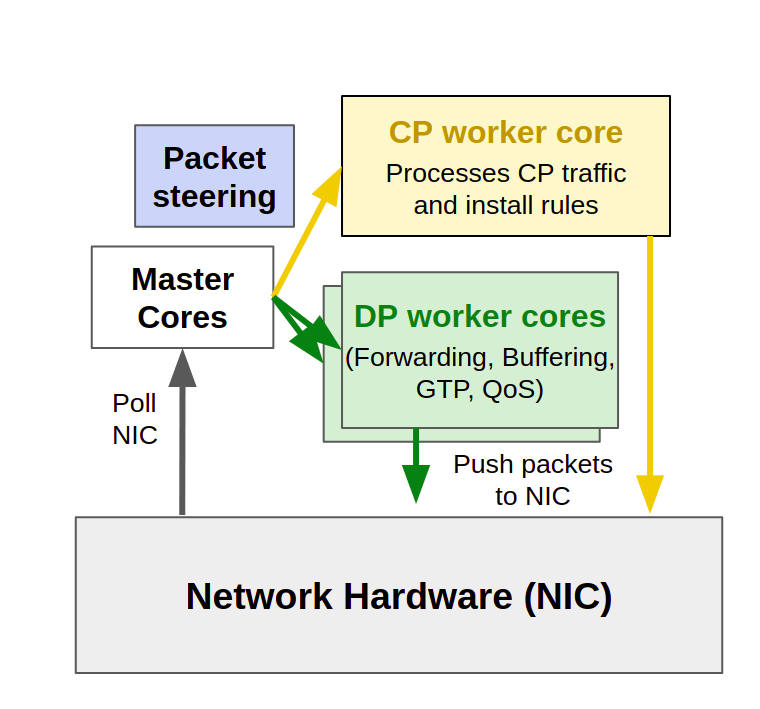
\includegraphics[width=70mm,height=50mm]{./fig/A.png}}
    \label{fig:DesignA}
    }
    \subfigure[]{
    \fbox{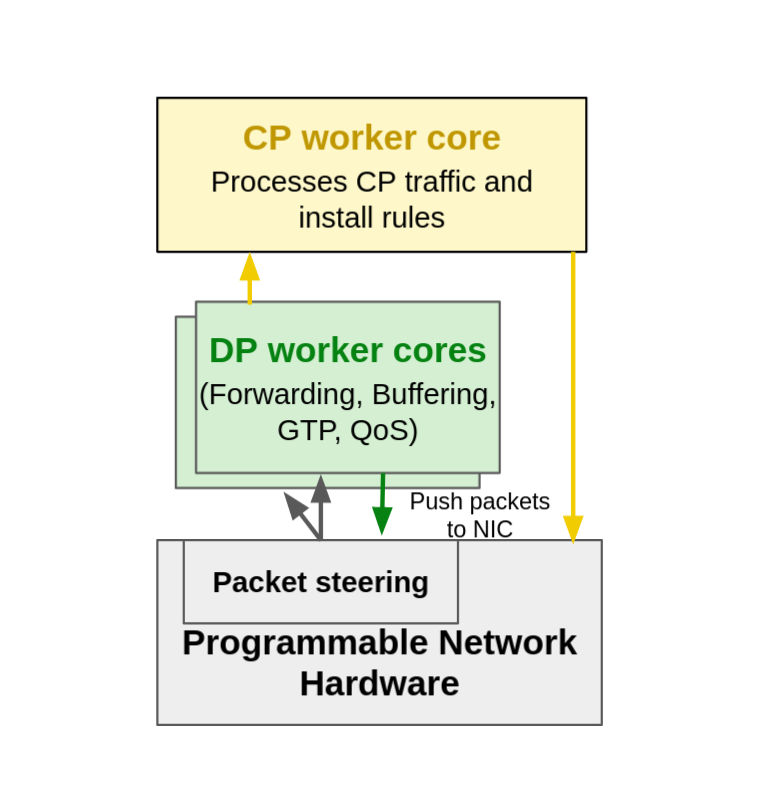
\includegraphics[width=70mm,height=50mm]{./fig/B.png}}
    \label{fig:DesignB}
    }
    
    \caption{\subref{fig:DesignA} Software UPF  \subref{fig:DesignB} SteerOffloaded Design}
        \label{figure:DesignAB}
    \end{figure}

\section{Evaluation}
\begin{figure}[htbp]
	\centering
	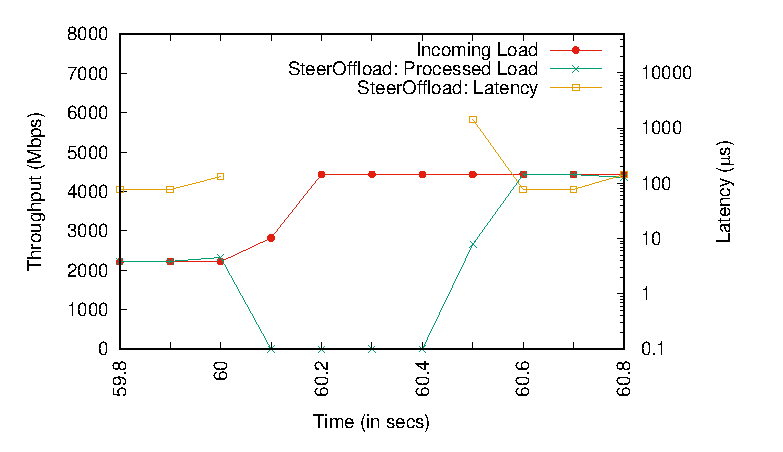
\includegraphics[width=0.7\textwidth]{fig/dynScaling_SteerOffload.eps}
	\setlength{\belowcaptionskip}{-12pt}
	\caption{SoftUPF vs. SteerOffload: Dynamic Scaling}
	\label{fig:dynamicScaling}
\end{figure}
\begin{figure}[htbp]
	\centering
	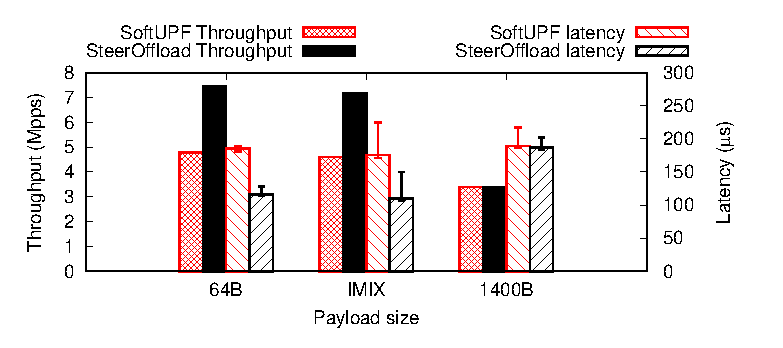
\includegraphics[width=0.7\textwidth]{fig/pipelineVsRTT.eps}
	%  \setlength{\abovecaptionskip}{-2pt}
	\setlength{\belowcaptionskip}{-12pt}

	\caption{SoftUPF vs. SteerOffload: Performance}
	
	\label{fig:UPFABperformance}
\end{figure}
\begin{figure}[htbp]
	\centering
	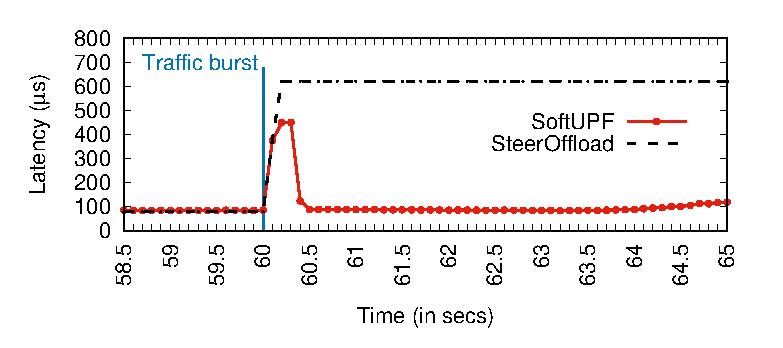
\includegraphics[width=0.7\textwidth]{fig/heavyHitter.eps}
	%  \setlength{\abovecaptionskip}{-2pt}
	\setlength{\belowcaptionskip}{-12pt}
	\caption{SoftUPF vs. SteerOffload: Heavy Hitters}
	\label{fig:HeavyHitter}
\end{figure}

